% Section 3.8: Data Flow and System Integration

\section{3.8 Data Flow and System Integration}
\label{sec:data-flow}
\addcontentsline{toc}{section}{3.8 Data Flow and System Integration}

\lettrine{T}{his section} examines how information flows through Symphony's architecture and how components integrate to form a cohesive system. We explore the directed acyclic graph model for workflow dependencies, the integration patterns that enable component collaboration, and the data governance mechanisms that ensure security and consistency. The data flow architecture provides the foundation for coordinating complex multi-step processes while maintaining clarity about data provenance and transformations.

\subsection*{3.8.1 Data Flow Model and Workflow Dependencies}
\addcontentsline{toc}{subsection}{3.8.1 Data Flow Model and Workflow Dependencies}

\lettrine{T}{he} data flow architecture of Symphony orchestrates the movement of information between components, ensuring that data reaches the right destinations at the right times while maintaining consistency and enabling efficient processing. The system treats data flow as a first-class concern, with explicit representations of how information moves through workflows and well-defined interfaces that govern data exchange between components. This architectural approach enables Symphony to coordinate complex multi-step processes involving numerous components while maintaining clarity about data provenance, transformations, and dependencies.

The conceptual data flow model represents workflows as directed acyclic graphs where nodes represent computational tasks and edges represent data dependencies between tasks. This graph-based representation makes explicit the flow of information through the system, enabling both automated reasoning about execution order and visual presentation that helps developers understand workflow structure. Each edge in the graph carries typed data, with the type system ensuring that data produced by one task is compatible with the expectations of tasks that consume it. This type safety prevents many common errors and enables early detection of incompatibilities before execution begins.

The workflow dependency management system analyzes the directed acyclic graph structure to determine valid execution orders that respect all dependencies. The topological sorting algorithm identifies a sequence in which tasks can execute such that each task runs only after all tasks it depends on have completed. When multiple valid execution orders exist, the system considers factors such as resource availability, task priorities, and opportunities for parallel execution to select an optimal order. This intelligent scheduling ensures that workflows execute efficiently while respecting all constraints and dependencies.

The overall system activity involves multiple components coordinating to process developer requests and generate outputs. The activity begins when a developer submits a prompt or selects a workflow to execute. The system analyzes the request to understand intent and identify required capabilities. The orchestration system generates or retrieves a workflow that accomplishes the objective. The execution engine processes the workflow, coordinating multiple extensions and managing data flow between them. Throughout execution, the system monitors progress, handles errors, and provides feedback to the developer. When execution completes, the system stores generated artifacts and updates its models based on the outcome. As illustrated in Figure 3.13, this complete activity flow demonstrates the coordination between all system components.

\begin{figure}[H]
\centering
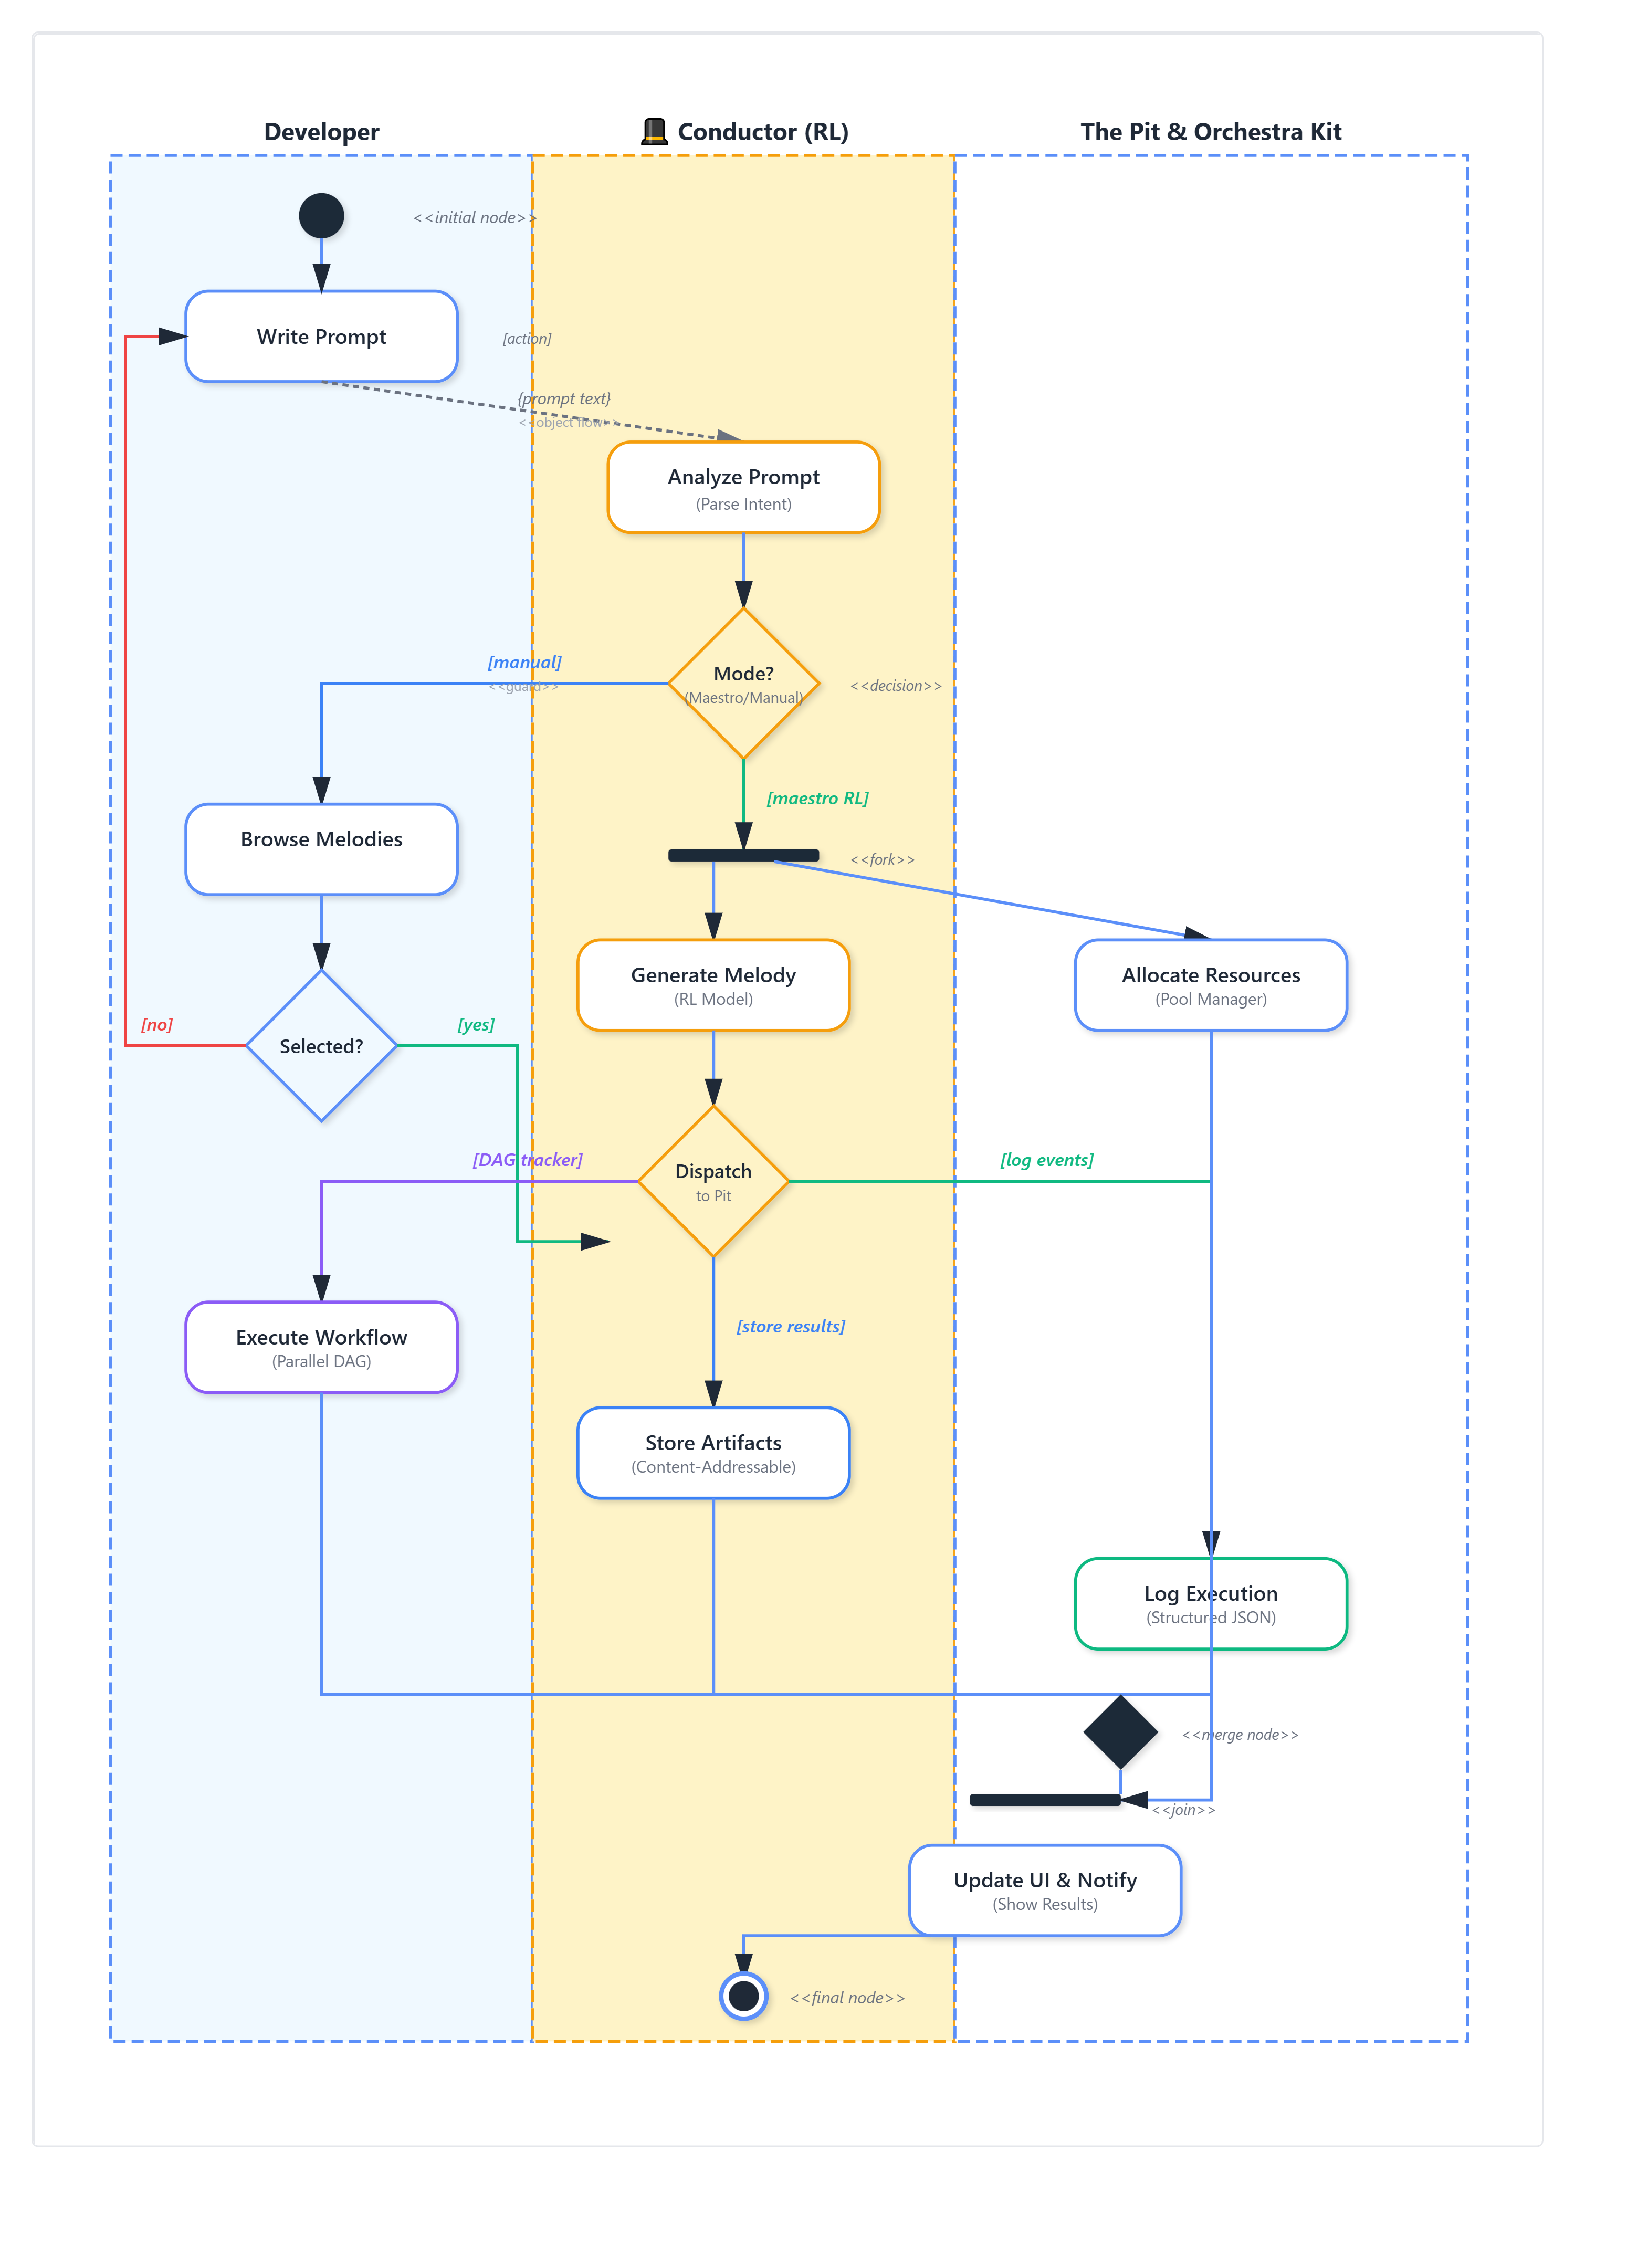
\includegraphics[width=0.95\textwidth]{images/diagrams/activity_diagram/symphony-activity-diagram.png}
\caption{Overall System Activity}
\label{fig:3.13-system-activity}
\end{figure}

\subsection*{3.8.2 Integration Patterns and Component Communication}
\addcontentsline{toc}{subsection}{3.8.2 Integration Patterns and Component Communication}

The integration patterns employed by Symphony enable components to work together effectively despite being developed independently and potentially using different technologies. The system defines clear interface contracts that specify how components communicate, what data formats they use, and what guarantees they provide. Components interact through these well-defined interfaces rather than depending on implementation details, enabling components to evolve independently as long as they continue to satisfy their interface contracts. This loose coupling between components facilitates system evolution and enables the extension ecosystem to grow without requiring coordination between extension developers.

The message passing infrastructure provides the foundation for component communication, implementing reliable delivery of messages between components regardless of whether they execute in the same process or in separate processes. The infrastructure handles serialization of complex data structures into formats suitable for transmission, routing of messages to appropriate destinations based on addressing information, buffering of messages when recipients are temporarily unavailable, and error handling when communication failures occur. This infrastructure abstracts away the complexities of inter-component communication, enabling components to focus on their domain logic rather than communication mechanics.

The data transformation capabilities enable components to work together even when they produce and consume data in different formats. The system provides a library of common transformations that convert between different representations, such as converting between different text encodings, transforming between different data structure formats, and adapting between different API conventions. Extensions can register custom transformations that handle domain-specific conversions, enabling seamless integration of specialized components. The transformation system applies conversions automatically when needed, making format differences transparent to workflow authors.

The system coordination principles that guide Symphony's integration architecture emphasize autonomy, loose coupling, and explicit contracts. Components should be autonomous, able to function independently without requiring tight coordination with other components. Components should be loosely coupled, depending on abstract interfaces rather than concrete implementations. Components should have explicit contracts that clearly specify their capabilities, requirements, and guarantees. These principles enable the system to scale to large numbers of components while maintaining understandability and reliability.

The event-driven architecture employed by Symphony enables components to react to system events without requiring tight coupling between event producers and consumers. Components can publish events to announce that interesting conditions have occurred, and other components can subscribe to events they care about without the publisher needing to know about subscribers. This publish-subscribe pattern enables flexible composition of behaviors, as new components can be added that react to existing events without modifying event publishers. The event system supports filtering and transformation, enabling subscribers to receive only relevant events in convenient formats.

The resource management system coordinates access to shared resources such as computational capacity, memory, storage, and external services. The system tracks resource availability and usage, enforces limits to prevent any component from monopolizing resources, implements fair allocation policies that ensure all components can make progress, and provides feedback to components about resource availability to enable adaptive behavior. This resource management ensures that the system remains responsive even under heavy load and that resources are allocated efficiently to maximize overall throughput.

\subsection*{3.8.3 Data Consistency and System Reliability}
\addcontentsline{toc}{subsection}{3.8.3 Data Consistency and System Reliability}

The error handling and recovery mechanisms ensure that the system remains stable and functional even when individual components encounter errors. The system implements fault isolation to prevent errors in one component from affecting others, automatic retry with exponential backoff for transient failures, graceful degradation when components become unavailable, and comprehensive logging to facilitate debugging and root cause analysis. These mechanisms ensure that Symphony provides a reliable platform for development even when dealing with the inherent unreliability of complex distributed systems.

The data consistency mechanisms ensure that information remains accurate and coherent as it flows through the system. The system implements transactional semantics for operations that must complete atomically, optimistic concurrency control for operations that rarely conflict, eventual consistency for operations where immediate consistency is not required, and conflict resolution strategies for situations where concurrent updates create inconsistencies. These mechanisms provide appropriate consistency guarantees for different types of operations while enabling high performance and availability.

The caching strategies employed throughout the system reduce latency and improve throughput by avoiding redundant computation and data retrieval. The system caches frequently accessed data close to where it is used, invalidates cached data when underlying sources change, implements cache warming to preload data that is likely to be needed, and applies eviction policies to manage cache size when memory is limited. These caching strategies significantly improve system responsiveness while ensuring that cached data remains accurate.

The monitoring and observability capabilities enable developers and system administrators to understand system behavior and diagnose issues. The system collects metrics about component performance, resource usage, error rates, and other operational characteristics. These metrics are aggregated and made available through dashboards and APIs that enable real-time monitoring and historical analysis. The system also implements distributed tracing that tracks requests as they flow through multiple components, enabling developers to understand the complete path of execution and identify bottlenecks or errors.

The integration testing framework enables verification that components work together correctly despite being developed independently. The framework provides tools for setting up test environments that include multiple components, generating test data that exercises integration points, asserting expected behaviors and outcomes, and cleaning up test environments after tests complete. This testing capability ensures that integration issues are caught early in the development process rather than manifesting as production failures.

The versioning and compatibility management system enables the extension ecosystem to evolve while maintaining stability for existing workflows. The system uses semantic versioning to communicate the nature of changes in new extension versions, maintains multiple versions of extensions to support workflows that depend on specific versions, provides compatibility shims that enable old workflows to work with new extension versions, and validates that workflow dependencies can be satisfied before execution begins. This versioning approach enables innovation while protecting existing workflows from breaking changes.

The data governance policies ensure that sensitive information is handled appropriately as it flows through the system. The system implements access controls that restrict which components can access sensitive data, audit logging that records all access to sensitive information, encryption for data at rest and in transit, and data retention policies that ensure information is not kept longer than necessary. These governance mechanisms enable Symphony to be used in environments with strict data handling requirements while maintaining the flexibility and power of the extension ecosystem.
